\item A maleta $A$ de \SI{15}{\kilogram} é liberada do repouso em $C$. Depois de deslizar por uma rampa lisa, atinge a maleta $B$ de \SI{10}{\kilogram} que está originalmente em repouso. Se o coeficiente de restituição entre maletas é $e=\SI{0.3}{}$, e o coeficiente de atrito cinético entro o solo $DE$ e cada maleta é $\mu_{k}=0.4$, determine: (a) a velocidade de $A$ imediatamente antes do impacto; (b) as velocidades de $A$ e $B$ logo após o impacto; e (c) a distância de $B$ desliza antes de entrar em repouso.

\begin{flushright}
	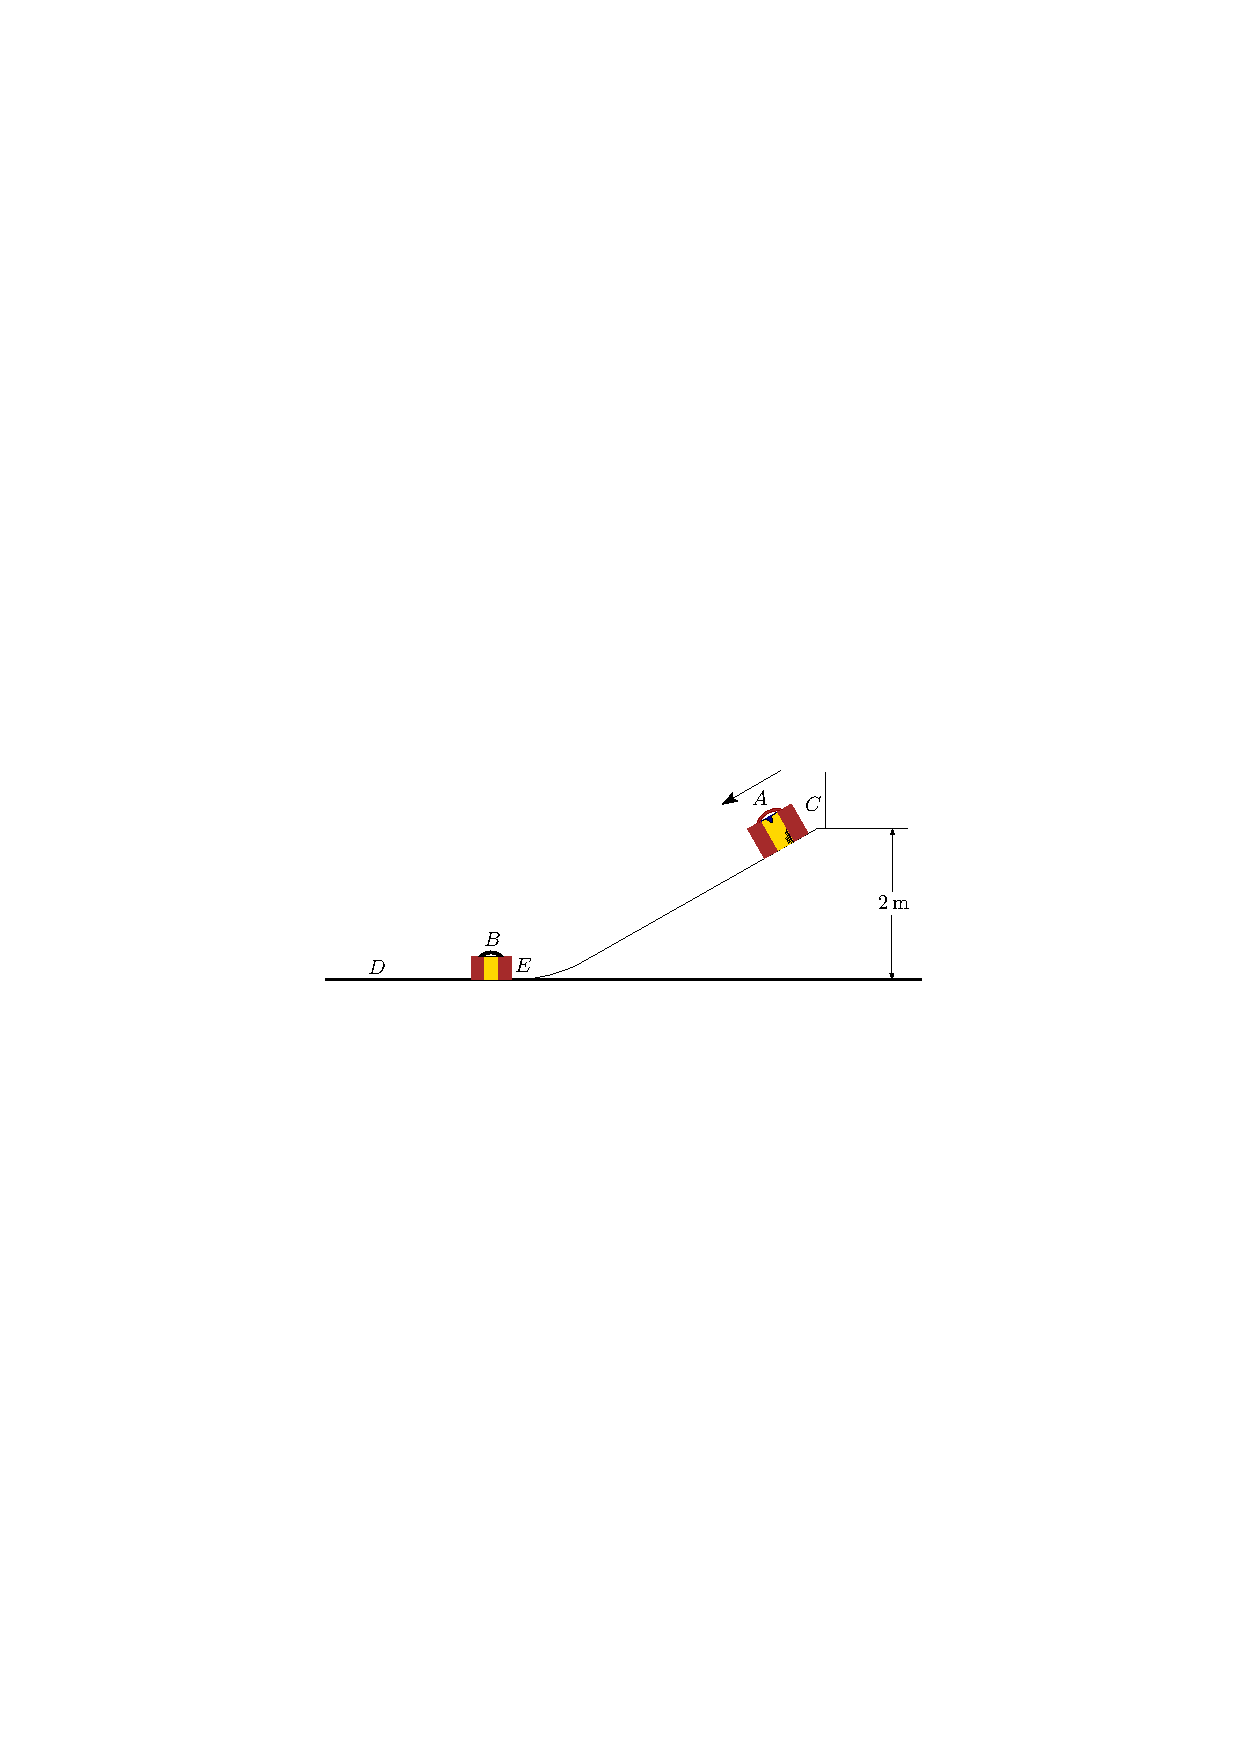
\includegraphics[scale=1.3]{images/draw_10}
\end{flushright}